\section{Metodologia}
\subsection{Densímetro}
    Neste experimento, um tubo rígido em forma de U deve ser parcialmente
    preenchido com água. Em uma das extremidades do tubo, é adicionado um
    líquido de densidade indeterminada, ao qual vamos nos referir como líquido
    misterioso. Então, após deixar o sistema entrar em equilíbrio, são anotadas
    as alturas das interfaces líquido-ar da água e do líquido misterioso em
    relação a interface líquido misterioso-água. O aparato montado com ambos os
    líquidos em equilíbrio pode ser observado na \cref{h2mist}
    
    \begin{figure}[H]
        \centering
        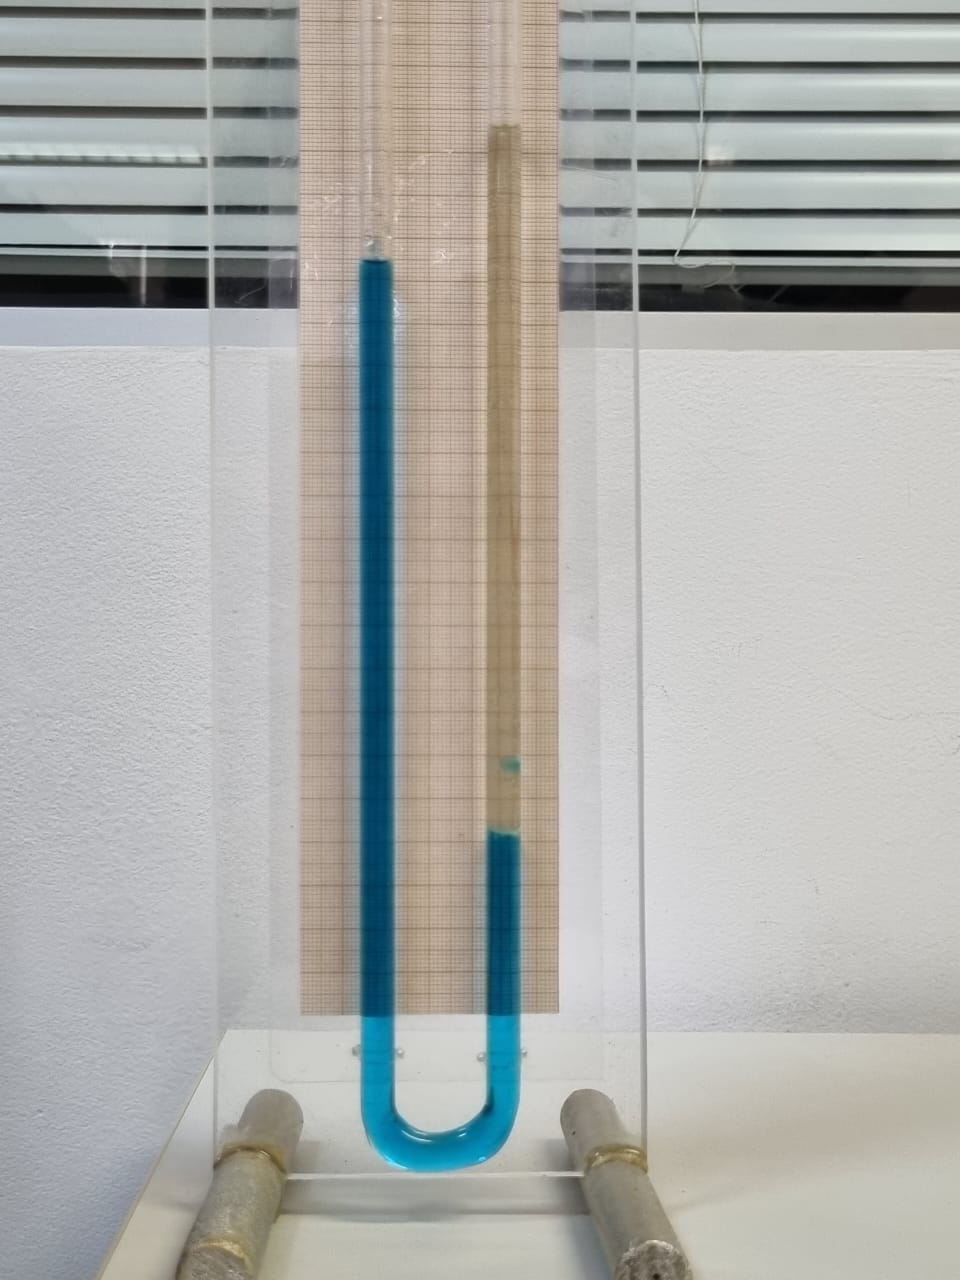
\includegraphics[width=0.25\linewidth]{fig/liquido_mis.jpeg}
        \caption{Tubo em U utilizado para determinar densidade do líquido
        misterioso}
        \label{h2mist}
    \end{figure}

\subsection{Manômetro}
    Para realização deste experimento é utilizado um manômetro de tubo aberto. O
    manômetro é constituido de um tubo rígido em forma de U com uma das
    extremidades aberta e a outra conectada a um tubo flexível. Ao lado do
    manômetro é disponibilizado um recipiente com água. O aparato pode ser
    observado na \cref{manometro} com a extremidade flexível submersa em água
    até a marcação de \(\qty{16}{cm}\). Para a tomada dos dados, criaremos a
    seguinte notação por conveniência:

    \begin{figure}[H]
        \centering
        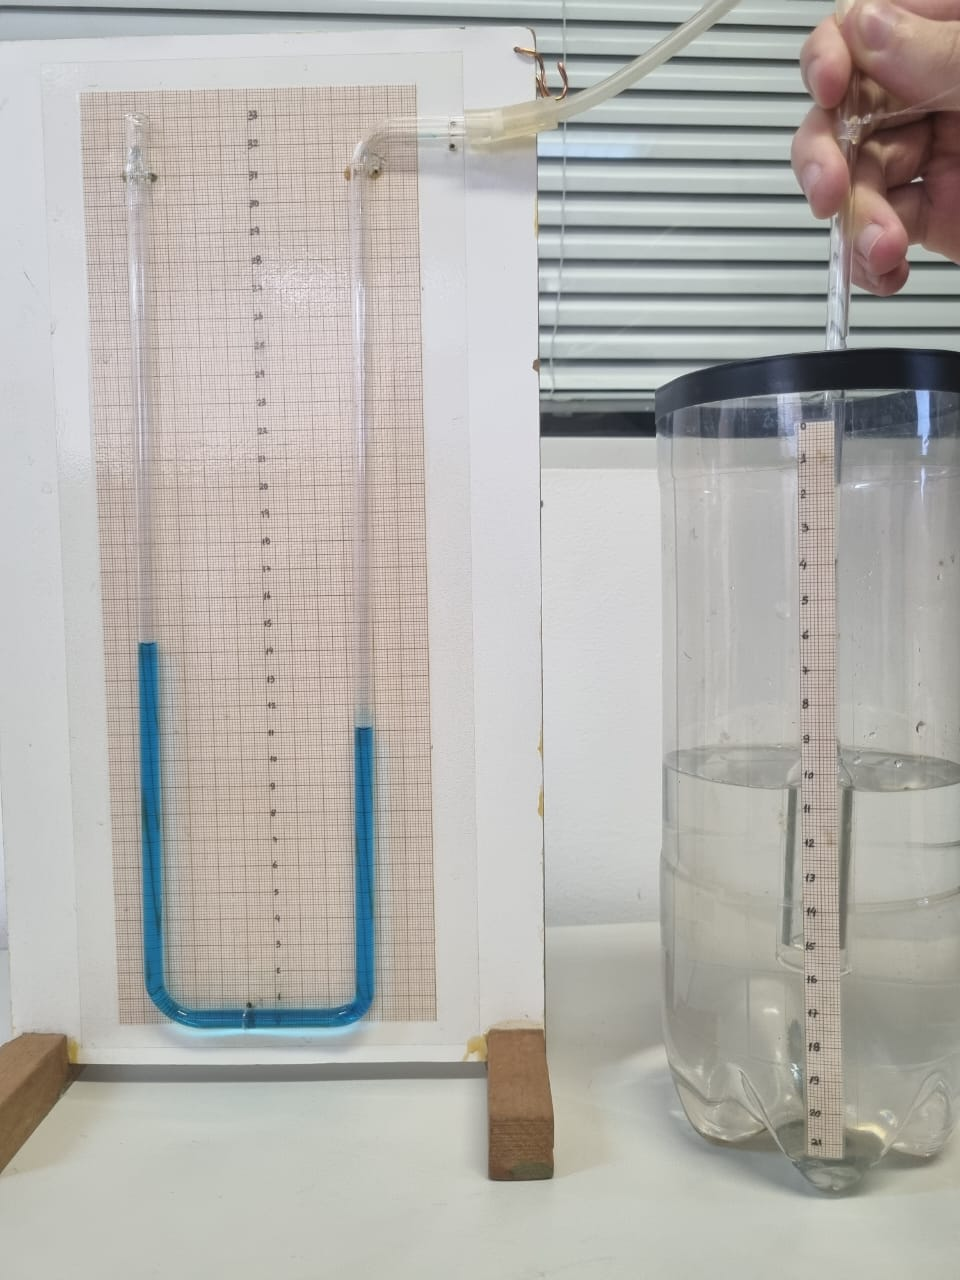
\includegraphics[width=0.25\textwidth]{fig/man_1.jpeg}
        \caption{manômetro de tubo aberto}
        \label{manometro}
    \end{figure}

    \begin{enumerate}
        \item Vamos nomear de Extremidade da Atmosfera, E. Atm, a ponta do tubo em U que está exposta ao ar;
        \item Vamos nomear de Extremidade do Recipiente, E. Conect, a ponta do tubo em U na qual se conecta o cano móvel a ser submerso no recipiente;
        \item Vamos nomear de Extremidade Livre, E. Livre, a ponta de vidro de diâmetro maior do cano móvel que submergimos no líquido;
    \end{enumerate}

    %TODO: arrumar tamanho da figura

    Para tomar uma medida, a E. Livre é submersa até a profundidade de interesse no recipiente e são anotadas as alturas dos pontos de interface líquido-ar na E. Atm e na E. Recip. Na \cref{manometro} é possível observar a tomada de medida do ponto de profundidade de \(\qty{16}{cm}\) do recipiente.

\subsection{Hemisférios de Magdeburg}

    Para este experimento, são utilizados dois pratos de borracha, cada um com \(\qty{0,35}{m}\) de diâmetro e área de \(\qty{0,0962}{m^2}\). Os dois pratos são alinhados e pressionados um contra o outro. Então, pode-se realizar força normal ao plano de interface entre os pratos. Uma maneira possível de exercer esta força é evidênciado na \cref{foto_hemisferio.png}.

\begin{figure}[H]
    \centering
    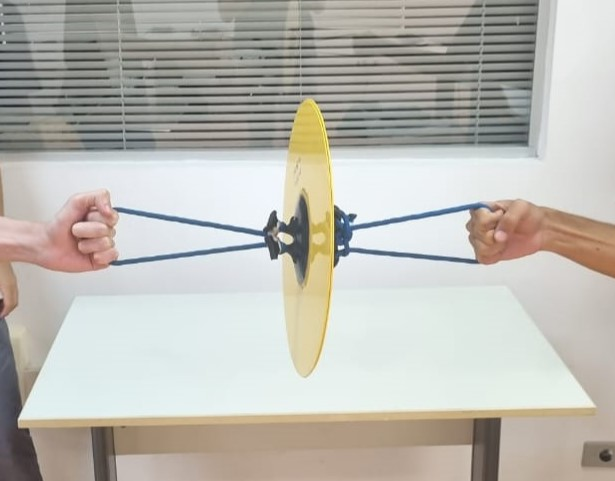
\includegraphics[width=0.25\textwidth]{fig/Cortada.jpeg}
    \caption{Dois estudantes fazendo força normal em sentidos opostos na tentativa de separar os hemisférios}
    \label{foto_hemisferio.png}
\end{figure}


\subsection{Equilíbrio de Pressões}
    No experimento ora descrito, são utilizados: um recipiente de vidro, uma membrana fina, um pedaço de cartolina e água. O recipiente tem a abertura coberta pela membrana e é parcialmente preenchido com água. Então, a cartolina é utilizada para cobrir a membrana. Por fim, o recipiente é virado rapidamente de ponta cabeça. Em seguida, a cartolina pode ser removida. Deve-se, então, observar o que ocorre com o líquido. Feito isto, pode-se observar o efeito de inclinar o recipiente, observando os fenômenos que levam a água a escorrer ou não. É possível observar o copo completamente na vertical e com a cartolina na \cref{c_c_v.png} e sem a cartolina, porém ligeiramente inclinado na \cref{c_m_i.png}.

    \begin{figure}[H]
        \centering
        \begin{subfigure}{.45\textwidth}
            \centering
            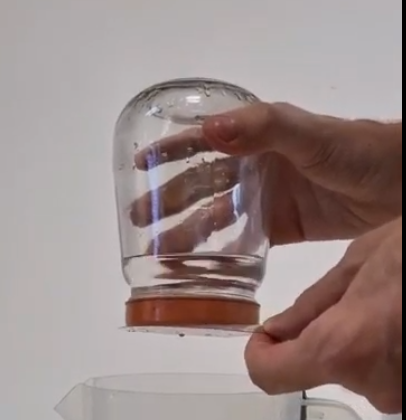
\includegraphics[width=0.5\linewidth]{fig/copo_cartolina.png}
            \caption{}
            \label{c_c_v.png}
        \end{subfigure}
        \begin{subfigure}{.45\textwidth}
            \centering
            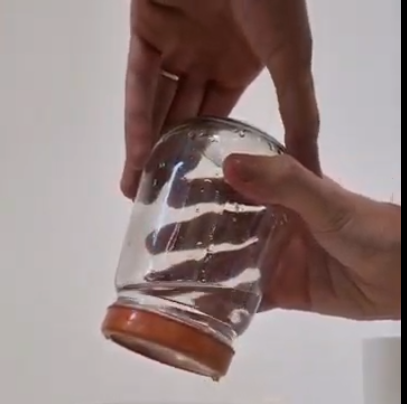
\includegraphics[width=.5\linewidth]{fig/copo_inclinado.png}
            \caption{}
            \label{c_m_i.png}
        \end{subfigure}
        \caption{Inclinação dos copos. (a) Copo com água de ponta cabeça com cartolina. (b) Copo com água sem cartolina virado de ponta cabeça e ligeiramente inclinado }
        \label{duasimage}
    \end{figure}

